\documentclass[11pt]{article}
\usepackage[utf8]{inputenc}
\usepackage[T1]{fontenc}
\usepackage[spanish,es-noshorthands]{babel}
\usepackage[margin=2.5cm]{geometry}
\usepackage{hyperref}
\hypersetup{colorlinks=true, linkcolor=blue, urlcolor=blue, citecolor=blue}
\usepackage{titlesec}
\usepackage{enumitem}
\usepackage{booktabs}
\usepackage{array}
\usepackage{tabularx}
\usepackage{parskip}
\usepackage{graphicx}
\usepackage{float}
\usepackage{caption}
\usepackage{amsmath}
\usepackage{textcomp}
\usepackage{tikz}
\usetikzlibrary{shapes.geometric, arrows.meta, positioning}

\titleformat{\section}{\large\bfseries}{\thesection}{1em}{}
\titleformat{\subsection}{\normalsize\bfseries}{\thesubsection}{1em}{}
\newcolumntype{Y}{>{\raggedright\arraybackslash}X}
\graphicspath{{img/}}

\title{\textbf{Informe Final \\ Ética y Seguridad de Datos (DS3031) -- Tipo 1}\\
\large Alzace Fitness: seguimiento de entrenamiento con privacidad diferencial}
\author{Joel M. Cayllahua Hilario \and Josué Renzo Hernández Yataco}
\date{\today}

\begin{document}
\maketitle

\begin{center}
\small Código: \url{https://github.com/Josu31506/Proyecto-2---etica-y-seguridad-de-datos}
\end{center}

\setcounter{tocdepth}{1}
\tableofcontents
\newpage

% ---------------------------------------------------------------
\section{Resumen}

Construimos una aplicación web para que Alzace Fitness acompañe a sus clientes de entrenamiento virtual. El cliente y su entrenador ven la ficha individual: mediciones, metas y sesiones. El club, en cambio, solo puede publicar una \textbf{estadística grupal protegida con privacidad diferencial}: los minutos activos promedio por persona y por mes.

Tres resultados principales:
\begin{itemize}[nosep]
  \item \textbf{Privacidad diferencial con $\varepsilon = 1$ por publicación.} En los datos de Fitbit, el error absoluto medio estimado con 30 semillas independientes es de \textbf{4,2 minutos} sobre una referencia de 34,05 min/día, y se devuelve un resultado en el 100\,\% de las simulaciones. La corrida con semilla fija que reproducen los notebooks da 4,7 minutos. Elegimos $\varepsilon = 1$ porque es el menor valor ensayado que cumple el objetivo fijado de antemano: error medio $\le 5$ minutos y al menos 95\,\% de respuestas. Ambas estimaciones lo cumplen.
  \item \textbf{Costo en el modelo.} Al entrenar un clasificador con ruido de Laplace ($\varepsilon = 1$), la exactitud bajó de 70,9\,\% a \textbf{69,1\,\%} en promedio sobre 30 semillas (unos $-1{,}8$ puntos; la corrida con semilla fija dio 68,4\,\%). En esa corrida la caída fue algo mayor en el grupo femenino ($-3{,}1$) que en el masculino ($-2{,}0$), y la brecha entre grupos pasó de 0,4 puntos a favor del grupo femenino a 0,7 a favor del masculino. Con estos tamaños de muestra la diferencia no es estadísticamente significativa (los intervalos de confianza de la exactitud de cada grupo se solapan casi por completo, una comparación aproximada): es una señal que hay que vigilar, no evidencia de sesgo.
  \item \textbf{Riesgo residual.} La DPIA identifica 9 riesgos a lo largo del ciclo de vida del dato. Después de las medidas implementadas, ninguno queda en nivel alto. Antes de un piloto con clientes reales quedan pendientes el despliegue con TLS, los plazos de conservación y un periodo de renovación del presupuesto $\varepsilon$ (sección~\ref{sec:cumplimiento}).
\end{itemize}

% ---------------------------------------------------------------
\section{Caso de negocio y KPIs}

Alzace Fitness pasa del entrenamiento presencial al virtual. Para no perder la supervisión, necesita registrar el progreso de cada cliente a distancia. Eso implica tratar \textbf{datos de salud} (frecuencia cardíaca, peso, grasa corporal y actividad), que la Ley N.\textdegree{}~29733 considera \textbf{datos sensibles} \cite{ley29733}.

Los KPIs propuestos en el parcial se implementaron en el panel (tabla~\ref{tab:kpis}).

\begin{table}[htbp]
\centering\small
\begin{tabularx}{\textwidth}{@{}p{4.2cm}Y@{}}
\toprule
\textbf{KPI} & \textbf{Cómo se calcula en la aplicación} \\
\midrule
Adherencia al plan & Sesiones de la semana marcadas como cumplidas entre sesiones programadas. \\
Progreso hacia la meta & Combinación de la fracción de minutos alcanzada y la reducción de grasa desde la primera medición del periodo. El entrenador fija los pesos y cada componente va de 0 a 100\,\%. \\
Retención & Membresías activas al inicio de un mes cerrado que siguen activas al final. \\
Tiempo de respuesta ante alertas & Tiempo medio del mes entre que se activa una alerta por sesión pendiente y su primera atención. \\
\bottomrule
\end{tabularx}
\caption{KPIs del caso de negocio.}
\label{tab:kpis}
\end{table}

La estadística grupal protegida responde a una necesidad distinta: que el club conozca la tendencia de actividad de sus clientes \textbf{sin} poder reconstruir la rutina de ninguno de ellos.

% ---------------------------------------------------------------
\section{Datos}

\begin{table}[htbp]
\centering\small
\begin{tabularx}{\textwidth}{@{}p{3.3cm}YY@{}}
\toprule
\textbf{Dataset} & \textbf{Contenido} & \textbf{Uso en el proyecto} \\
\midrule
\href{https://www.kaggle.com/datasets/arashnic/fitbit}{Fitbit Fitness Tracker Data} & 33 participantes y 940 días-persona de actividad diaria, del 12 de abril al 12 de mayo de 2016. & Estadística protegida con privacidad diferencial y su experimento de utilidad. \\
\href{https://www.kaggle.com/datasets/valakhorasani/gym-members-exercise-dataset}{Gym Members Exercise} & 973 perfiles con edad, género, experiencia, frecuencia, duración de sesión, etc. & Modelo de clasificación con y sin protección, y análisis de sesgo. \\
\bottomrule
\end{tabularx}
\caption{Fuentes de datos.}
\end{table}

\textbf{Decisiones sobre los datos:}
\begin{itemize}[nosep]
  \item \textbf{Usamos solo la exportación de abril--mayo de Fitbit.} La exportación anterior (marzo--abril) tiene fechas solapadas con valores contradictorios. La importación verifica conflictos y se detiene si los encuentra.
  \item \textbf{Abandonamos el vínculo aleatorio Fitbit--Gym propuesto en el parcial.} Las fuentes no comparten un identificador de persona, así que unirlas al azar produciría ``clientes'' que no existen y conclusiones sin validez. Cada fuente se analiza por separado (sección~\ref{sec:lecciones}).
  \item \textbf{El identificador de Fitbit se seudonimiza} con HMAC-SHA-256 y una clave independiente antes de guardarse. Las identidades de la demo son ficticias.
\end{itemize}

\begin{figure}[htbp]
\centering
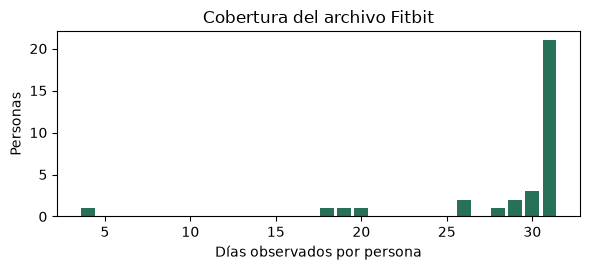
\includegraphics[width=0.75\textwidth]{cobertura-fitbit.png}
\caption{Días observados por persona en todo el archivo de Fitbit (12 de abril a 12 de mayo de 2016). La mayoría tiene entre 28 y 31 días, pero algunas personas registran muy pocos (mínimo 4). Promediar por fila haría que las personas con más días pesen más; por eso la estadística da un voto a cada persona.}
\label{fig:cobertura}
\end{figure}

% ---------------------------------------------------------------
\section{Implementación}

\begin{table}[htbp]
\centering\small
\begin{tabularx}{\textwidth}{@{}p{2.4cm}p{3.6cm}Y@{}}
\toprule
\textbf{Capa} & \textbf{Tecnología} & \textbf{Qué hace} \\
\midrule
Frontend & Next.js & Pantallas separadas para Cliente (actividad, historial, importar CSV, privacidad), Entrenador (clientes asignados, metas, sesiones, alertas) y Administrador (estadísticas, auditoría, operaciones). \\
Backend & FastAPI (Python) & Autorización por rol y por registro, cifrado, privacidad diferencial, presupuesto $\varepsilon$, auditoría y respaldos. \\
Base de datos & SQLite (demo) y PostgreSQL con esquema privado (modo alojado) & Fichas cifradas, publicaciones, presupuesto y eventos de auditoría. \\
Análisis & 3 notebooks de Jupyter & Exploración, experimento de privacidad diferencial y modelo + ética. Usan las mismas funciones que el backend. \\
\bottomrule
\end{tabularx}
\caption{Arquitectura del prototipo.}
\end{table}

\begin{center}
\resizebox{\textwidth}{!}{%
\begin{tikzpicture}[
  box/.style={rectangle, rounded corners, draw=black!60, fill=green!8, text width=2.9cm, align=center, minimum height=1.1cm, font=\scriptsize, inner sep=3pt},
  dark/.style={box, fill=teal!25},
  arr/.style={-{Latex[length=1.8mm]}, thick, black!70}
]
  \node[box] (web) at (0,0) {\textbf{Web (Next.js)}\\ vistas por rol};
  \node[box] (api) at (4,0) {\textbf{API (FastAPI)}\\ valida rol y propietario};
  \node[dark] (enc) at (8,0) {\textbf{Cifrado}\\ AES-256-GCM por campo};
  \node[box] (db) at (12,0) {\textbf{Base de datos}\\ fichas cifradas};
  \node[dark] (dp) at (8,-1.7) {\textbf{Laplace} ($\varepsilon=1$)\\ + cargo de presupuesto};
  \node[box] (pub) at (12,-1.7) {\textbf{Publicación guardada}\\ la lee el entrenador};
  \draw[arr] (web) -- (api);
  \draw[arr] (api) -- (enc);
  \draw[arr] (enc) -- (db);
  \draw[arr] (api) |- (dp) node[pos=0.25, left, font=\tiny] {admin publica};
  \draw[arr] (dp) -- (pub);
\end{tikzpicture}%
}
\end{center}

% ---------------------------------------------------------------
\section{Privacidad diferencial}
\label{sec:dp}

\subsection{Qué se publica}
La pregunta es: \emph{¿cuántos minutos activos por día registró, en promedio, una persona del grupo en los días observados del mes?} El archivo no cubre meses completos: abril de 2016 solo tiene datos del 12 al 30 (19 días) y mayo, del 1 al 12. La \textbf{unidad protegida es la persona}: dos bases vecinas se diferencian en \textbf{todos} los registros de un participante, no solo en un día.

Usamos la definición estándar \cite{dwork2014}: un mecanismo aleatorio $M$ es $\varepsilon$-diferencialmente privado si, para cualquier par de bases vecinas $D$ y $D'$ y cualquier conjunto de resultados $R$,
\[
\Pr[M(D) \in R] \;\le\; e^{\varepsilon}\,\Pr[M(D') \in R].
\]
Es decir, que una persona esté o no en los datos cambia la probabilidad de cualquier resultado como máximo en un factor $e^{\varepsilon}$.

\subsection{Mecanismo}
\begin{enumerate}[nosep]
  \item Por cada día se suman los minutos de actividad moderada e intensa.
  \item Se calcula la media de cada participante en sus días observados y se acota a $[0, 120]$ minutos.
  \item Se centra en 60 minutos. Así, añadir o quitar a una persona cambia la suma como máximo en 60 y el conteo en 1.
  \item Se aplican \textbf{dos mecanismos de Laplace independientes}, con $\varepsilon/2 = 0{,}5$ cada uno: uno a la suma (escala 120) y otro al conteo (escala 2). Por composición secuencial, la publicación es $(\varepsilon = 1, \delta = 0)$-DP.
  \item Si el conteo \textbf{con ruido} es menor que 8, se omite el valor. El cálculo $60 + \tilde{S}/\tilde{n}$, la acotación y el redondeo son posprocesamiento, así que no consumen presupuesto.
\end{enumerate}

\[
\tilde{S} = \sum_i (x_i - 60) + \mathrm{Lap}\!\left(\frac{60}{0{,}5}\right), \qquad
\tilde{n} = n + \mathrm{Lap}\!\left(\frac{1}{0{,}5}\right), \qquad
\hat{\mu} = 60 + \frac{\tilde{S}}{\tilde{n}}
\]

Implementación: \texttt{backend/privacy.py}.

\subsection{Presupuesto}
La instalación tiene un \textbf{presupuesto global de $\varepsilon = 2$}, o sea, dos publicaciones distintas. El cargo del $\varepsilon$ y la publicación se guardan \textbf{en la misma transacción}. Si se pide otra vez el mismo mes y la misma fuente, se devuelve el resultado guardado \textbf{sin gastar $\varepsilon$}. Así se evita el ataque de promediar muchas respuestas con ruido nuevo. Lo comprobamos en la demo: dos publicaciones de abril de 2016 dieron el mismo valor (32,5 min) y el gasto se quedó en 1,0 de 2,0.

\textbf{Un presupuesto fijo no alcanza para seguir una tendencia.} Con $\varepsilon = 2$ en total y $\varepsilon = 1$ por publicación, la instalación puede publicar solo dos meses en toda su vida. En la demo lo dejamos así a propósito, para mostrar que el presupuesto se agota y que la API rechaza la tercera publicación. Para un piloto habría que definir un periodo de renovación, por ejemplo un presupuesto anual. Renovar no borra lo ya publicado: por composición, la pérdida de privacidad de una persona que sigue en los datos se suma periodo tras periodo (con $\varepsilon = 2$ al año, al cabo de tres años serían $\varepsilon = 6$). Ese total acumulado tiene que declararse en la documentación y en el consentimiento. Fijar el periodo queda como decisión pendiente del responsable (tabla~\ref{tab:pendientes}).

\subsection{Elección de la librería}
\label{sec:libreria}
Elegimos \textbf{IBM diffprivlib 0.6.6} \cite{holohan2019} porque:
\begin{itemize}[nosep]
  \item permite declarar la sensibilidad y repartir el presupuesto de forma explícita;
  \item las mismas operaciones sirven en la API y en el experimento;
  \item su mecanismo de Laplace usa un muestreo diseñado para evitar los ataques por precisión finita de los números de punto flotante \cite{holohan2021}.
\end{itemize}
La definición de la unidad protegida, los límites y la composición siguen siendo responsabilidad del equipo, como recomienda la guía NIST SP 800-226 \cite{nist800226}.

Antes de decidir comparamos diffprivlib con otras librerías abiertas conocidas (tabla~\ref{tab:librerias}). La comparación es general: no hicimos pruebas de rendimiento con las otras opciones.

\begin{table}[htbp]
\centering\small
\begin{tabularx}{\textwidth}{@{}p{2.3cm}p{2.4cm}YYY@{}}
\toprule
\textbf{Librería} & \textbf{Lenguaje} & \textbf{Mecanismos y herramientas} & \textbf{Contabilidad del presupuesto} & \textbf{Orientación} \\
\midrule
\textbf{IBM diffprivlib} \cite{holohan2019} & Python & Laplace, Gauss, exponencial y otros; funciones al estilo de NumPy y modelos compatibles con scikit-learn. & Contador de presupuesto opcional (\texttt{BudgetAccountant}). & Investigación y prototipos en Python. \\
OpenDP & Núcleo en Rust, con interfaz para Python & Mediciones y transformaciones que se combinan, con mapas de privacidad verificables. & Combinadores de composición y \emph{odómetros}. & Proyecto comunitario de origen académico; muy expresivo, pero con una curva de aprendizaje mayor. \\
Google Differential Privacy & C++, Java y Go (en Python, mediante envoltorios de terceros) & Agregaciones acotadas (conteo, suma, media) con Laplace y Gauss; Privacy on Beam para flujos de datos. & Se asigna por agregación o por flujo. & Procesamiento de datos a gran escala. \\
Tumult Analytics & Python, sobre Apache Spark & Consultas de agregación sobre tablas, al estilo SQL. & Sesión con presupuesto total que se descuenta en cada consulta. & Publicación de estadísticas sobre grandes volúmenes. \\
\bottomrule
\end{tabularx}
\caption{Comparación general de librerías de privacidad diferencial.}
\label{tab:librerias}
\end{table}

Nos quedamos con diffprivlib porque el proyecto es pequeño y está escrito en Python. Se integra directamente con NumPy y scikit-learn, que ya usábamos en los notebooks y en el modelo. Además, está documentada en una publicación revisable \cite{holohan2019}. OpenDP y Tumult serían alternativas razonables si el servicio creciera, pero su complejidad o su dependencia de Spark no se justifican para una estadística mensual de unas decenas de personas.

\subsection{Elección de \texorpdfstring{$\varepsilon$}{epsilon}: experimento de utilidad}
\label{sec:epsilon}
En abril de 2016 (datos del 12 al 30) hay 33 participantes y 611 días-persona, con entre 4 y 19 días por persona. Como referencia, la media por persona acotada es \textbf{34,05 min/día}. Para cada valor de $\varepsilon$ simulamos 300 publicaciones (tabla~\ref{tab:eps}).

\begin{table}[htbp]
\centering\small
\begin{tabular}{@{}rrrr@{}}
\toprule
\textbf{$\varepsilon$ por publicación} & \textbf{Resultados devueltos} & \textbf{Error absoluto medio} & \textbf{Percentil 90 del error} \\
\midrule
0,1 & 83,7\,\% & 30,3 min & 67,9 min \\
0,5 & 99,7\,\% & 9,5 min & 19,6 min \\
\textbf{1} & \textbf{100\,\%} & \textbf{4,7 min} & \textbf{9,7 min} \\
2 & 100\,\% & 2,3 min & 4,7 min \\
\bottomrule
\end{tabular}
\caption{Utilidad de la estadística según $\varepsilon$ (Fitbit, abril de 2016; 300 simulaciones por valor).}
\label{tab:eps}
\end{table}

\begin{figure}[htbp]
\centering
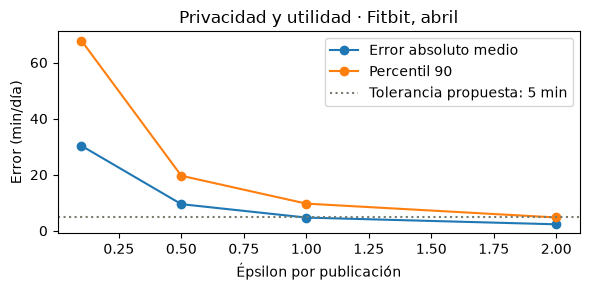
\includegraphics[width=0.75\textwidth]{privacidad-utilidad-fitbit.png}
\caption{Error de la estadística según $\varepsilon$. $\varepsilon = 1$ es el primer valor ensayado que cumple el criterio de error medio $\le 5$ minutos. Subir a $\varepsilon = 2$ reduce el error a la mitad (de 4,7 a 2,3 min), pero duplica la pérdida de privacidad de cada publicación.}
\end{figure}

\textbf{Interpretación:}
\begin{itemize}[nosep]
  \item Con $\varepsilon = 1$, una publicación típica se desvía unos \textbf{5 minutos de 34 ($\approx$\,14\,\%)}. Basta para ver si la actividad del grupo sube o baja, pero \textbf{no} para tomar decisiones sobre una persona. Por eso la interfaz muestra la unidad y el periodo de cada estimación.
  \item Con $\varepsilon = 0{,}1$ se omite el resultado en el 16\,\% de los casos y el error es de casi la misma magnitud que la media: más privacidad, pero la estadística deja de ser útil.
  \item La protección tiene \textbf{otros costos además del ruido}. Acotar la contribución de cada persona baja la referencia de 34,69 a 34,05 min/día y subestima a las personas más activas. Dar un voto por persona, en vez de uno por fila (35,49), también cambia la cifra. Lo documentamos en vez de ocultarlo.
\end{itemize}

\textbf{Lectura desde la privacidad.} El criterio de utilidad no basta: también hay que preguntarse qué protege $\varepsilon = 1$. Según la definición, incluir o excluir a una persona cambia la probabilidad de cualquier resultado publicado como máximo en un factor $e^{1} \approx 2{,}72$. Con el presupuesto total de la instalación ($\varepsilon = 2$, dos publicaciones), el factor máximo es $e^{2} \approx 7{,}4$. No existe un valor ``correcto'' universal. Lee y Clifton \cite{lee2011} muestran que el mismo $\varepsilon$ implica riesgos de identificación distintos según los datos, y Hsu et al. \cite{hsu2014} proponen elegirlo equilibrando el costo para los participantes con el valor de la estadística, que es la lógica que seguimos aquí. En la práctica tampoco hay un valor estándar, y algunos despliegues grandes usan presupuestos muy superiores a 1. El Censo de EE.UU. adoptó la privacidad diferencial para 2020 \cite{abowd2018}; su presupuesto final para los datos de redistritación, repartido entre muchas tablas y expresado en zCDP, equivale a $\varepsilon = 17{,}14$ para las tablas de personas y $\varepsilon = 2{,}47$ para las de viviendas \cite{census2021,abowd2022}. Nuestro $\varepsilon = 1$ por publicación y $\varepsilon = 2$ en total son mucho más conservadores que ese ejemplo, aunque protegen una sola estadística y no un censo completo.

% ---------------------------------------------------------------
\section{Utilidad para modelado}
\label{sec:modelo}

Para medir el efecto de la privacidad en un modelo, entrenamos un clasificador sobre Gym que predice si una sesión dura \textbf{al menos 75 minutos}, a partir del nivel de experiencia y la frecuencia semanal. Datos: 681 filas de entrenamiento y 292 de prueba.
\begin{itemize}[nosep]
  \item \textbf{Referencia:} un histograma de 21 combinaciones $\times$ 2 clases.
  \item \textbf{Versión privada:} el mismo histograma con ruido de Laplace (sensibilidad $L_1 = 1$, porque una fila cambia una sola celda), 30 entrenamientos por cada $\varepsilon$. Aquí la unidad protegida es \textbf{una fila}, porque Gym no tiene un identificador de persona a lo largo del tiempo.
\end{itemize}

\begin{table}[htbp]
\centering\small
\begin{tabular}{@{}lrr@{}}
\toprule
\textbf{Resultado en prueba} & \textbf{Sin protección} & \textbf{Con $\varepsilon = 1$ (media de 30)} \\
\midrule
Exactitud & 70,9\,\% & 68,4\,\% \\
Exactitud balanceada & 69,4\,\% & 68,8\,\% \\
AUC del ataque de inferencia de membresía & 0,492 & 0,493 \\
Exactitud, grupo femenino ($n = 128$) & 71,1\,\% & 68,0\,\% \\
Exactitud, grupo masculino ($n = 164$) & 70,7\,\% & 68,7\,\% \\
\bottomrule
\end{tabular}
\caption{Clasificador de duración de sesión en Gym, con y sin privacidad diferencial.}
\end{table}

\begin{figure}[htbp]
\centering
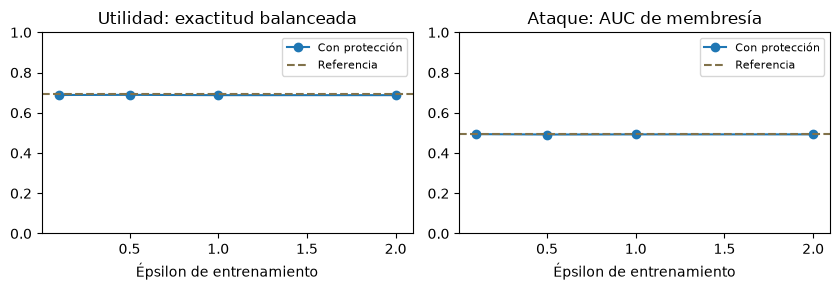
\includegraphics[width=0.9\textwidth]{modelo-gym.png}
\caption{La exactitud balanceada y el ataque de membresía casi no cambian con $\varepsilon$.}
\end{figure}

\textbf{Interpretación:}
\begin{itemize}[nosep]
  \item \textbf{El costo en utilidad es bajo:} $-2{,}5$ puntos de exactitud y $-0{,}65$ puntos de exactitud balanceada con la semilla fija; con 30 semillas, la caída de exactitud es de unos $-1{,}8$ puntos.
  \item \textbf{El ataque de membresía \cite{shokri2017} no funciona en ninguna de las dos versiones} (AUC $\approx 0{,}49$, o sea, azar). Un modelo de 42 conteos casi no memoriza filas individuales, así que en este caso \textbf{no pudimos demostrar empíricamente} que la privacidad diferencial reduzca el riesgo. La garantía sigue siendo la matemática de la sección~\ref{sec:dp}.
  \item \textbf{Limitación detectada y cómo la tratamos:} en la tabla, $\varepsilon = 1$ y $\varepsilon = 2$ dan resultados idénticos. La tabla es una corrida con semilla fija, que los notebooks reproducen exactamente, y esa semilla se reutiliza para cada $\varepsilon$: el ruido tiene siempre el mismo signo y la caída viene de unas pocas celdas casi empatadas que el ruido voltea sin importar su tamaño. Por eso tomamos como estimación de referencia la de 30 semillas independientes por $\varepsilon$ (sección~\ref{sec:robustez}): con $\varepsilon = 1$, la exactitud privada es de 69,1\,\% y el costo, de unos $-1{,}8$ puntos. Las dos estimaciones llevan a la misma conclusión.
\end{itemize}

\subsection{Robustez de los experimentos}
\label{sec:robustez}
Los valores principales de este informe salen de una sola semilla por experimento, que además se reutiliza para todos los $\varepsilon$. Para comprobar que las conclusiones no dependen de esa semilla, repetimos ambos experimentos con \textbf{30 semillas independientes}, distintas para cada $\varepsilon$ y cada repetición, usando las mismas funciones de \texttt{backend/experiment.py} y \texttt{backend/privacy.py}. En Fitbit, cada semilla corresponde a 300 publicaciones simuladas, como en el experimento principal. También repetimos la estadística con los datos de mayo de 2016 y con topes de 90 y 150 minutos en lugar de 120. La tabla~\ref{tab:robustez} muestra la media del error absoluto medio entre semillas, su desviación estándar y el intervalo de confianza al 95\,\% de esa media (distribución $t$ con 29 grados de libertad). El cálculo se reproduce con \texttt{scripts/robustez.py} y sus resultados quedan en \texttt{evidence/robustez.json}.

\begin{table}[htbp]
\centering\small
\begin{tabular}{@{}lrrrrr@{}}
\toprule
\textbf{Escenario} & \textbf{Referencia} & \textbf{$\varepsilon = 0{,}1$} & \textbf{$\varepsilon = 0{,}5$} & \textbf{$\varepsilon = 1$} & \textbf{$\varepsilon = 2$} \\
\midrule
Abril, tope 120 (principal) & 34,05 & 27,5 $\pm$ 1,1 & 8,3 $\pm$ 0,4 & \textbf{4,2 $\pm$ 0,2} & 2,0 $\pm$ 0,1 \\
\quad IC95 de la media & & [27,1; 27,9] & [8,1; 8,4] & [4,1; 4,3] & [2,0; 2,1] \\
\quad Valor con la semilla fija (tabla~\ref{tab:eps}) & & 30,3 & 9,5 & 4,7 & 2,3 \\
Mayo, tope 120 & 31,86 & 28,1 $\pm$ 1,3 & 9,3 $\pm$ 0,6 & 4,6 $\pm$ 0,2 & 2,3 $\pm$ 0,1 \\
Abril, tope 90 & 32,74 & 20,8 $\pm$ 0,9 & 5,9 $\pm$ 0,3 & 2,9 $\pm$ 0,2 & 1,5 $\pm$ 0,1 \\
Abril, tope 150 & 34,69 & 33,5 $\pm$ 1,8 & 10,9 $\pm$ 0,5 & 5,5 $\pm$ 0,3 & 2,7 $\pm$ 0,2 \\
\bottomrule
\end{tabular}
\caption{Error absoluto medio (minutos) de la estadística de Fitbit: media $\pm$ desviación estándar entre 30 semillas independientes. Con $\varepsilon \ge 0{,}5$ se devolvió un resultado en al menos el 99\,\% de las simulaciones de cada semilla, en todos los escenarios. Mayo solo tiene datos del 1 al 12 (30 personas y 329 días-persona).}
\label{tab:robustez}
\end{table}

\textbf{Lo que muestra el análisis:}
\begin{itemize}[nosep]
  \item \textbf{La semilla fija era pesimista.} Los valores de la tabla~\ref{tab:eps} no caen dentro del intervalo de confianza: con $\varepsilon \ge 0{,}5$ quedan incluso algo por encima del máximo observado entre las 30 semillas (con $\varepsilon = 1$, 4,7 frente a un rango de 3,7 a 4,6). Como la semilla se reutiliza, la misma ``mala suerte'' se repite, escalada, en todos los $\varepsilon$. El error real esperado con $\varepsilon = 1$ es de unos 4,2 minutos, así que los valores principales sobrestiman el error en torno a un 13\,\%. La conclusión no cambia, porque el sesgo va en la dirección conservadora.
  \item \textbf{La elección de $\varepsilon = 1$ se sostiene con abril y con mayo}: en las 30 semillas el error medio quedó bajo 5 minutos (máximo 4,6 en abril y 4,9 en mayo), y con $\varepsilon = 0{,}5$ nunca se cumplió el criterio. En mayo el margen es menor porque hay menos personas y menos días.
  \item \textbf{La elección de $\varepsilon$ depende del tope.} El tope de 120 minutos se fijó antes del experimento como parámetro público del mecanismo (\texttt{LIMIT} en \texttt{backend/privacy.py}) y no lo cambiamos a la vista de estos resultados: elegirlo según los datos también tendría un costo de privacidad, que habría que contabilizar. Lo que sí muestra el análisis es que, con un tope de 150 minutos, la sensibilidad crece y $\varepsilon = 1$ ya no cumple el criterio (5,5 minutos). Con 90 minutos el ruido baja a 2,9, pero la referencia se aleja más de la media sin acotar (32,74 frente a 34,69). Ese sesgo no aparece en la tabla, porque el error se mide contra la referencia ya acotada de cada escenario, así que estos datos no bastan para decir qué tope es el mejor.
  \item \textbf{Modelo de Gym.} Con semillas independientes, la exactitud privada con $\varepsilon = 1$ es de $69{,}1 \pm 0{,}4$\,\% (IC95 [68,9; 69,2]; rango de 67,9 a 69,8), y con $\varepsilon = 2$ de $69{,}2 \pm 0{,}4$\,\%. El valor principal (68,4\,\%) cae dentro del rango, pero por debajo del intervalo: también aquí la semilla fija fue algo pesimista, y el costo real ronda los $-1{,}8$ puntos y no los $-2{,}5$. Además, $\varepsilon = 1$ y $\varepsilon = 2$ ya no son idénticos, aunque la diferencia es muy pequeña.
\end{itemize}
El script de este análisis queda fuera del código del servicio y no altera el archivo \path{evidence/experimentos.json}.

% ---------------------------------------------------------------
\section{Evaluación de impacto (DPIA)}
\label{sec:dpia}

\subsection{Descripción del tratamiento}
\begin{table}[htbp]
\centering\small
\begin{tabularx}{\textwidth}{@{}p{3.3cm}Y@{}}
\toprule
\textbf{Elemento} & \textbf{Detalle} \\
\midrule
Responsable & Alzace Fitness (el club). El entrenador actúa solo sobre sus clientes asignados. El operador técnico custodia las claves, los respaldos y el presupuesto $\varepsilon$. \\
Encargados previstos & Supabase (base de datos y autenticación) y Render (API y web) para el despliegue. Ambos alojan los datos fuera del Perú (ver transferencia internacional). \\
Titulares & Clientes del entrenamiento virtual. En la demo son personas ficticias; los participantes de Fitbit son datos de estudio. \\
Datos & Identificación (nombre, correo), actividad diaria, sueño, frecuencia cardíaca, peso y \% de grasa, metas y sesiones. \\
Categoría legal & \textbf{Datos sensibles (salud)} según la Ley 29733 \cite{ley29733}: exigen consentimiento \textbf{por escrito} y medidas de seguridad reforzadas. \\
Finalidad principal & Acompañar el entrenamiento que el cliente solicitó. \\
Finalidad secundaria & Estimar tendencias grupales de actividad. Es \textbf{opcional}: requiere consentimiento propio y empieza desactivada. \\
\bottomrule
\end{tabularx}
\caption{Descripción del tratamiento evaluado.}
\label{tab:tratamiento}
\end{table}

\subsection{Transferencia internacional}
En el modo alojado, Supabase y Render guardarían y procesarían los datos en centros de datos fuera del Perú. Eso es un \textbf{flujo transfronterizo de datos personales}, que la Ley 29733 y su Reglamento regulan \cite{ley29733}: el país o el destinatario deben ofrecer un nivel de protección adecuado, o el responsable debe garantizarlo por otros medios. Medidas previstas:
\begin{itemize}[nosep]
  \item \textbf{Cifrado antes de salir:} las mediciones se cifran por campo en la API, y las claves no se guardan en el proveedor de base de datos. Supabase solo almacena texto cifrado.
  \item \textbf{Contrato de encargo} con cada proveedor, que limite el uso de los datos a la prestación del servicio y obligue a notificar incidentes. Hay que elegir la región de alojamiento y documentarla.
  \item \textbf{Transparencia:} el consentimiento debe informar que los datos se alojan fuera del país y con qué proveedores.
  \item \textbf{Modo demo local:} la demostración y las pruebas usan SQLite en el equipo del grupo con personas ficticias, así que hoy no hay transferencia. Antes del piloto hay que revisar las obligaciones de comunicación a la ANPD que fije el Reglamento.
\end{itemize}

\subsection{Necesidad y proporcionalidad}
\begin{itemize}[nosep]
  \item \textbf{Minimización:} la estadística grupal usa solo los minutos activos, no el peso ni la frecuencia cardíaca. El panel de administración \textbf{no muestra} historias biométricas.
  \item \textbf{Limitación de la finalidad:} el permiso de un estudio no autoriza a contactar a sus participantes ni a convertirlos en clientes. Los datos de Fitbit solo alimentan la estadística del estudio.
  \item \textbf{Base legal:} el seguimiento individual se basa en la relación con el servicio y en el consentimiento expreso para datos de salud. La analítica grupal se basa en un consentimiento \textbf{separado y revocable}. Negarse no afecta el acceso al plan.
  \item \textbf{Alternativa menos invasiva:} se descartó el vínculo Fitbit--Gym, porque crearía perfiles inexistentes sin ningún beneficio para el titular.
\end{itemize}

\subsection{Riesgos a lo largo del ciclo de vida}
\textbf{Método.} Cada riesgo se califica por probabilidad (P) e impacto (I) en una escala de tres niveles: B = bajo (1), M = medio (2), A = alto (3). El nivel es el producto P $\times$ I: \textbf{bajo} si vale 1 o 2, \textbf{medio} si vale 3 o 4, y \textbf{alto} si vale 6 o 9. El riesgo residual se calcula igual, con la probabilidad y el impacto que quedan después de las medidas: una medida puede bajar la probabilidad (por ejemplo, un control de acceso probado) o el impacto (por ejemplo, el cifrado o un presupuesto que acota la pérdida). La categoría sigue LINDDUN \cite{linddun}.

\begin{table}[htbp]
\centering\small
\begin{tabularx}{\textwidth}{@{}l>{\raggedright\arraybackslash}p{2.1cm}Y>{\raggedright\arraybackslash}p{2.4cm}ccc@{}}
\toprule
\textbf{\#} & \textbf{Etapa} & \textbf{Escenario de riesgo} & \textbf{LINDDUN} & \textbf{P} & \textbf{I} & \textbf{Inicial} \\
\midrule
R1 & Acceso & Un entrenador o cliente consulta la ficha de otro cliente (IDOR) & Disclosure & M & A & \textbf{Alto} \\
R2 & Estadística & Comparar promedios publicados permite reconocer la rutina de una persona & Linkability, Identifiability & M & A & \textbf{Alto} \\
R3 & Estadística & Republicar el mismo mes con ruido nuevo hasta promediarlo & Disclosure & M & A & \textbf{Alto} \\
R4 & Recolección & Participar en la estadística se percibe como condición del servicio & Non-compliance, Unawareness & M & A & \textbf{Alto} \\
R5 & Conservación & Robo de la base o de un respaldo con datos de salud en claro & Disclosure & M & A & \textbf{Alto} \\
R6 & Preparación & Fechas y patrones de actividad permiten reidentificar a pesar del seudónimo & Linkability & M & M & Medio \\
R7 & Uso & Una predicción sesgada cambia el plan de una persona & Ética: sesgo & M & A & \textbf{Alto} \\
R8 & Estadística & Personas con pocos días quedan subrepresentadas, o el tope subestima a las muy activas & Ética: sesgo & A & B & Medio \\
R9 & Respaldo & Restaurar un respaldo antiguo ``devuelve'' presupuesto ya gastado & Disclosure & B & A & Medio \\
\bottomrule
\end{tabularx}
\caption{Riesgos identificados.}
\end{table}

\subsection{Medidas y riesgo residual}
\begin{table}[htbp]
\centering\small
\begin{tabularx}{\textwidth}{@{}lY>{\raggedright\arraybackslash}p{3.3cm}>{\raggedright\arraybackslash}p{2.3cm}cc@{}}
\toprule
\textbf{\#} & \textbf{Medida implementada} & \textbf{Cómo se verifica} & \textbf{Responsable} & \textbf{P/I} & \textbf{Residual} \\
\midrule
R1 & La API autoriza \textbf{cada objeto} por rol y por propietario, y audita las denegaciones. & Probado: el cliente recibe 403 al pedir la ficha de otro; el entrenador recibe 403 con un cliente no asignado. & Equipo de backend & B/A & Medio \\
R2 & Privacidad diferencial $\varepsilon = 1$ a nivel de persona, aporte acotado y umbral sobre el conteo con ruido. & Prueba de sensibilidad, experimento de 300 simulaciones y análisis con 30 semillas independientes. & Responsable de analítica & B/A & Medio \\
R3 & Presupuesto global $\varepsilon = 2$, cargo y publicación en la misma transacción, resultado guardado. & Probado: publicar dos veces devuelve el mismo valor y no gasta más $\varepsilon$. & Operador técnico & B/M & Bajo \\
R4 & Pantalla de consentimiento con el propósito explicado, opción desactivada por defecto, retiro y registro de la preferencia. & Recorrido en ``Mi privacidad''. & Responsable del club & B/M & Bajo \\
R5 & Cifrado AES-256-GCM por campo, con datos asociados (tabla, propietario, fecha, versión de clave). Respaldo cifrado con otra clave. Rotación de claves. & Una manipulación invalida el descifrado. Pruebas de respaldo y verificación. & Operador técnico & M/M & Medio \\
R6 & Seudónimo HMAC con clave separada. Los CSV originales quedan fuera de Git y de los paneles. & Revisión del repositorio y \texttt{.gitignore}. & Equipo de datos & M/M & Medio \\
R7 & El modelo se queda en el notebook (laboratorio). Revisión humana obligatoria y comparación de utilidad por grupo. & Sección~\ref{sec:modelo}. & Entrenador y equipo de datos & B/M & Bajo \\
R8 & Promedio por persona. El efecto del tope se cuantifica y se publica (34,69 $\rightarrow$ 34,05). & Secciones~\ref{sec:dp} y~\ref{sec:robustez}. & Equipo de datos & A/B & Medio \\
R9 & Procedimiento operativo (no automatizado): tras restaurar un respaldo, y antes de publicar, el operador compara el gasto registrado con las publicaciones ya divulgadas y no publica si no coinciden. & \texttt{backup verify} comprueba que el gasto coincide con las publicaciones del propio respaldo. La comparación con lo divulgado es manual. & Operador técnico & B/A & Medio \\
\bottomrule
\end{tabularx}
\caption{Medidas, responsables y riesgo residual (P/I residuales).}
\end{table}

Justificaciones de la calificación residual:
\begin{itemize}[nosep]
  \item En R1 y R2 las medidas bajan la probabilidad, pero el impacto sigue siendo alto porque una falla expondría datos de salud; por eso quedan en medio.
  \item En R3 el presupuesto acota la pérdida máxima ($\varepsilon = 2$ en total), lo que reduce el impacto. En R5 el cifrado reduce el impacto de un robo, pero la probabilidad no cambia. En R7 la revisión humana impide que una predicción cambie un plan por sí sola.
  \item R6 sigue en medio porque el seudónimo impide recuperar el identificador original, pero no cambia las fechas ni los patrones diarios, que son justamente lo que permite vincular a una persona. No generalizamos las fechas porque el seguimiento individual las necesita. Las medidas reducen dónde circulan los datos, no lo que revelan.
  \item R8 sigue en medio porque el tope y el voto por persona son parte del método: se aplican en cada publicación (en abril, el tope afectó a una persona), así que la probabilidad no baja. Lo que hacemos es cuantificar y publicar el efecto. El impacto ya era bajo, porque la cifra es grupal y no se usa para decidir sobre nadie.
  \item En R9 la medida es un procedimiento manual y no baja la probabilidad ni el impacto: el residual es igual al inicial. La probabilidad ya era baja, porque restaurar un respaldo antiguo es una operación excepcional, y el impacto sigue alto porque se podría superar el presupuesto declarado sin que nadie lo note. Automatizar esa comparación queda pendiente (tabla~\ref{tab:pendientes}).
\end{itemize}

\subsection{Consulta a los afectados}
Hasta ahora no consultamos a clientes reales, porque la demo usa personas ficticias. Antes del piloto, el responsable del club enviará un \textbf{aviso a los socios} que explique qué datos se tratarán, la estadística grupal, el carácter opcional del consentimiento y el alojamiento fuera del país. Con el aviso irá una \textbf{encuesta breve} que pregunte si se entiende la pantalla de consentimiento, si alguien se siente obligado a participar y qué usos les preocupan. Además, se hará una prueba de la pantalla ``Mi privacidad'' con un grupo pequeño de socios. Los resultados se incorporarán a esta DPIA y, si es necesario, cambiarán las medidas.

\subsection{Decisión}
\textbf{Se puede pilotar con condiciones.} Ningún riesgo residual queda en nivel alto. Antes de incorporar clientes reales hay que:
\begin{enumerate}[nosep]
  \item desplegar con TLS en ambos extremos (Supabase y Render), firmar los contratos de encargo y documentar la región de alojamiento;
  \item definir un plazo de conservación y una vía de eliminación verificable, incluidas las copias;
  \item designar a quién atiende las solicitudes ARCO. La aplicación todavía no permite que el cliente exporte o borre sus propios datos; mientras tanto, esas solicitudes se atenderían de forma manual, y automatizarlas queda como trabajo futuro;
  \item inscribir el banco de datos ante la ANPD;
  \item realizar la consulta a los socios descrita arriba;
  \item ensayar un incidente con el equipo, incluida la comunicación a la ANPD dentro del plazo de 48 horas que establece el Reglamento aprobado por el D.S. 016-2024-JUS \cite{ley29733}.
\end{enumerate}

% ---------------------------------------------------------------
\section{Reflexiones éticas}
\label{sec:etica}

\subsection*{Sesgo algorítmico}
\begin{itemize}[nosep]
  \item \textbf{Observamos una diferencia entre grupos, pero no es evidencia de sesgo.} Con $\varepsilon = 1$, la exactitud del grupo femenino bajó de 71,1\,\% a 68,0\,\% ($-3{,}1$ puntos) y la del masculino de 70,7\,\% a 68,7\,\% ($-2{,}0$). La brecha pasó de 0,4 puntos a favor del grupo femenino a 0,7 a favor del masculino, es decir, cambió alrededor de 1,1 puntos. Sin embargo, con 128 y 164 personas en el conjunto de prueba, el error estándar de la exactitud de cada grupo es de unos 4 puntos (unos 5,4 para la diferencia entre ambos). Los intervalos de confianza de Wilson al 95\,\% para la exactitud de cada grupo son, sin protección, [62,7; 78,2] para el femenino y [63,4; 77,2] para el masculino, y con protección, aproximadamente [59,5; 75,4] y [61,2; 75,3]. Se solapan casi por completo, y una brecha final de 0,7 puntos queda muy por debajo del error estándar de la diferencia, así que no es estadísticamente significativa. Hay que leer estos intervalos con cuidado: se refieren al nivel de exactitud de cada grupo, no a la diferencia entre sus caídas. Las dos versiones del modelo se evalúan sobre el mismo conjunto de prueba, así que las caídas están pareadas, y compararlas con estos intervalos es solo una aproximación; no hicimos una prueba pareada. En términos absolutos, la caída equivale a unas 4 filas del grupo femenino y unas 3 del masculino. Con semillas independientes (sección~\ref{sec:robustez}) la brecha también es pequeña: 68,8\,\% frente a 69,3\,\%.
  \item Aun así, es una \textbf{observación que hay que vigilar}. Bagdasaryan et al. \cite{bagdasaryan2019} muestran que la privacidad diferencial puede perjudicar más a los grupos con menos datos. Lo tomamos como un motivo para medir la utilidad por grupo cada vez que se entrene un modelo, no como la explicación demostrada de lo que vimos aquí. Para detectar diferencias de este tamaño harían falta muchos más datos.
  \item Las categorías de género del dataset (solo dos) dejan fuera otras identidades. El tamaño de los grupos tampoco permite conclusiones fuertes.
  \item \textbf{``Un día sin reloj no es un día inactivo''.} Por eso la adherencia se calcula con sesiones declaradas como cumplidas, no con días sin registro. Si no, se castigaría a quien no tiene un wearable.
\end{itemize}

\subsection*{Transparencia}
\begin{itemize}[nosep]
  \item Publicamos el método, la unidad protegida, el $\varepsilon$ y el error esperado (sección~\ref{sec:dp}), incluidos los costos del tope y del voto por persona.
  \item La interfaz presenta cada estadística con su unidad y su periodo. Así se evita que alguien la lea como un dato individual.
\end{itemize}

\subsection*{Consentimiento}
\begin{itemize}[nosep]
  \item El consentimiento para la analítica es \textbf{separado, opcional, desactivado por defecto y revocable}. El cliente no pierde su plan si se niega.
  \item Retirarlo afecta a las consultas futuras, pero \textbf{no borra} lo ya publicado. Lo explicamos en la pantalla, porque un consentimiento solo es informado si la persona sabe qué no se puede deshacer.
\end{itemize}

\subsection*{Tensión de fondo}
Más privacidad ($\varepsilon$ pequeño) da una estadística inútil para el club. Menos privacidad expone a las personas. Elegimos $\varepsilon = 1$ con un criterio de utilidad y un tope de 120 minutos \textbf{fijados antes} de mirar los resultados, y limitamos el número de publicaciones. Desde el lado de la privacidad, ese valor significa que la presencia de una persona puede cambiar la probabilidad de un resultado como máximo en un factor de 2,72 por publicación (7,4 con el presupuesto total), mucho menos que, por ejemplo, el presupuesto del Censo de EE.UU. de 2020 (sección~\ref{sec:epsilon}). La decisión se puede revisar, pero queda documentada y no es arbitraria.

% ---------------------------------------------------------------
\section{Seguridad y verificación}

\begin{table}[htbp]
\centering\small
\begin{tabularx}{\textwidth}{@{}p{3cm}Y@{}}
\toprule
\textbf{Medida} & \textbf{Implementación} \\
\midrule
Cifrado en reposo & AES-256-GCM por campo, nonce de 96 bits y etiqueta autenticada. \\
Contraseñas & bcrypt con coste 12 y sal individual. En el modo alojado, Supabase Auth. \\
Sesiones & Cookie HttpOnly y SameSite=Strict (Secure en el modo alojado). Verificación del origen y de un encabezado propio en las escrituras. \\
Autorización & Por rol y por registro, validada en el servidor. \\
Auditoría & Eventos de solo inserción: sesiones, publicaciones, importaciones, denegaciones. \\
Respaldos & Copia cifrada con una clave distinta y verificación por restauración en memoria. \\
En tránsito & En el modo alojado la configuración \textbf{exige} HTTPS y \texttt{sslmode=verify-full} hacia PostgreSQL. Si falta, no arranca. \\
Escaneo & OWASP ZAP 2.17 \cite{zap} pasivo con los 4 roles: 38 mensajes y \textbf{solo 3 alertas informativas}, ninguna de riesgo bajo, medio o alto. \\
\bottomrule
\end{tabularx}
\caption{Medidas de seguridad implementadas.}
\end{table}

\textbf{Pruebas ejecutadas} (26/11/2026, en un equipo del grupo con Windows y Python 3.13):
\begin{itemize}[nosep]
  \item \texttt{pytest}: \textbf{12 pruebas pasan}. 1 se omite porque requiere una base PostgreSQL de pruebas, definida en la variable \texttt{ALZACE\_TEST\_PG}. Incluyen acceso a fichas ajenas (403), presupuesto agotado (409), meses no cerrados (422), auditoría de rechazos y supresión de la retención en cohortes pequeñas.
  \item Playwright (navegador): \textbf{5 pruebas de extremo a extremo pasan} (cliente, entrenador, administrador, acceso a datos ajenos y agotamiento del presupuesto).
  \item Next.js compila en modo producción.
  \item Los 3 notebooks se ejecutan de principio a fin, y el experimento reproduce exactamente los resultados guardados en \texttt{evidence/experimentos.json}.
  \item Recorrido en vivo por la API: acceso cruzado denegado (403); escritura sin encabezado propio rechazada (403); publicación repetida sin gasto adicional de $\varepsilon$; evento de auditoría de la publicación registrado (\texttt{estadistica.\allowbreak publicar}).
\end{itemize}

% ---------------------------------------------------------------
\section{Cumplimiento de requerimientos}
\label{sec:cumplimiento}

\begin{table}[htbp]
\centering\small
\begin{tabularx}{\textwidth}{@{}p{6cm}cY@{}}
\toprule
\textbf{Requerimiento del enunciado final} & \textbf{Estado} & \textbf{Evidencia} \\
\midrule
Evaluar riesgos de privacidad y éticos & Cumplido & Secciones~\ref{sec:dpia} y~\ref{sec:etica} \\
Mantener la utilidad para análisis y modelado & Cumplido & Error de 4,2 min (4,7 con semilla fija); unos $-1{,}8$ puntos de exactitud ($-2{,}5$ con semilla fija) \\
Implementar y evaluar privacidad diferencial & Cumplido & Sección~\ref{sec:dp}, \texttt{backend/privacy.py}, notebook 02 \\
Justificar la librería y $\varepsilon$ con evidencia & Cumplido & Secciones~\ref{sec:libreria}, \ref{sec:epsilon} y~\ref{sec:robustez}, referencias \\
DPIA del ciclo de vida & Cumplido & Sección~\ref{sec:dpia} \\
Ética: sesgo, transparencia y consentimiento & Cumplido & Sección~\ref{sec:etica} \\
Al menos una base de datos & Cumplido & SQLite (demo) y PostgreSQL (modo alojado) \\
Front y backend & Cumplido & Next.js y FastAPI \\
Notebooks & Cumplido & \texttt{notebooks/01--03} \\
\bottomrule
\end{tabularx}
\caption{Cumplimiento del enunciado final.}
\end{table}

\textbf{Lo que no se logró y por qué:}
\begin{table}[htbp]
\centering\small
\begin{tabularx}{\textwidth}{@{}p{5cm}Y@{}}
\toprule
\textbf{Pendiente} & \textbf{Justificación} \\
\midrule
Despliegue en Supabase + Render con TLS (prometido en el parcial) & La configuración está lista y exige HTTPS y \texttt{verify-full}, pero no llegamos a validar el staging con cuentas del equipo a tiempo. La demo es local, por eso \textbf{no evaluamos TLS en producción}. \\
Prueba de concurrencia sobre PostgreSQL & Existe (\texttt{tests/test\_postgres.py}), pero necesita una base de pruebas externa. Se omitió en esta ejecución. \\
Escaneo ZAP activo & Solo se ejecutó el pasivo. El activo debe hacerse con autorización sobre el staging. \\
Plazo de conservación y eliminación verificable & Está planteado en la DPIA y es condición antes del piloto. \\
Exportar o borrar los datos propios desde la aplicación & No está implementado. Por ahora las solicitudes ARCO se atenderían de forma manual; queda como trabajo futuro. \\
Periodo de renovación del presupuesto $\varepsilon$ & En la demo el presupuesto es global y fijo a propósito (dos publicaciones en total). Un piloto necesita un periodo de renovación y declarar la pérdida acumulada entre periodos (sección~\ref{sec:dp}). \\
Comparar el presupuesto con lo divulgado al restaurar (R9) & Hoy es un procedimiento manual. \texttt{backup verify} solo comprueba la coherencia interna del respaldo. \\
\bottomrule
\end{tabularx}
\caption{Pendientes y su justificación.}
\label{tab:pendientes}
\end{table}

% ---------------------------------------------------------------
\section{Conclusiones}
\begin{enumerate}[nosep]
  \item \textbf{La privacidad diferencial es viable para la estadística del club.} Con $\varepsilon = 1$, el error medio es de unos 4,2 minutos sobre 34 (4,7 en la corrida con semilla fija), suficiente para ver si la actividad del grupo sube o baja sin exponer a nadie. El valor de $\varepsilon$ se eligió con un criterio fijado antes del experimento. Para seguir una tendencia en el tiempo hace falta, además, renovar el presupuesto por periodos y declarar la pérdida acumulada.
  \item \textbf{El costo para el modelado fue bajo} (unos $-1{,}8$ puntos con 30 semillas independientes y $-2{,}5$ con la semilla fija). La brecha entre grupos pasó de 0,4 puntos a favor del grupo femenino a 0,7 a favor del masculino; con este tamaño de muestra, esa diferencia no es estadísticamente significativa. No es evidencia de sesgo, pero sí una señal que vigilar: proteger la privacidad y ser justo con todos los grupos son objetivos que hay que medir por separado.
  \item \textbf{La privacidad no es solo ruido.} Las decisiones que más protegen fueron de diseño: la unidad protegida (la persona), el presupuesto con resultados guardados, el consentimiento separado, no mostrar datos individuales al administrador y descartar un vínculo de datos sin fundamento.
  \item \textbf{Lo que falta es operativo:} despliegue con TLS, conservación, ARCO y la renovación del presupuesto $\varepsilon$. Por eso la decisión de la DPIA es ``pilotar con condiciones'', no ``lanzar''.
\end{enumerate}

% ---------------------------------------------------------------
\section{Lecciones aprendidas y retrospectiva}
\label{sec:lecciones}
\begin{itemize}[nosep]
  \item \textbf{Cambiar el diseño cuando los datos no lo sostienen.} En el parcial propusimos unir Fitbit y Gym al azar. Al implementarlo vimos que generaba personas inexistentes, así que lo descartamos y analizamos cada fuente por separado.
  \item \textbf{Definir la unidad protegida es lo más difícil.} Proteger ``una fila'' o ``una persona'' cambia la sensibilidad y la garantía. En Fitbit pudimos proteger a la persona; en Gym, solo la fila.
  \item \textbf{Un experimento también puede tener errores de diseño.} Usar la misma semilla para todos los $\varepsilon$ hizo indistinguibles $\varepsilon = 1$ y $\varepsilon = 2$ en el modelo. Lo detectamos al reproducir los resultados y lo complementamos con 30 semillas independientes, que mostraron que la semilla fija daba cifras algo pesimistas (sección~\ref{sec:robustez}).
  \item \textbf{El presupuesto $\varepsilon$ es un recurso que se acaba.} Durante las pruebas gastamos la mitad del presupuesto de la demo y tuvimos que reiniciar la base antes de presentarla. En un servicio real, esto obliga a planificar qué preguntas valen la pena.
  \item \textbf{Retrospectiva de equipo.} La implementación avanzó en un solo repositorio, y la verificación, el informe y la presentación se cerraron al final. Para otro proyecto, conviene revisar entregables y código en paralelo desde el inicio, y no concentrar la documentación en la última semana.
\end{itemize}

% ---------------------------------------------------------------
\begin{thebibliography}{99}
\bibitem{dwork2014} C. Dwork y A. Roth. \emph{The Algorithmic Foundations of Differential Privacy}. Foundations and Trends in Theoretical Computer Science, 2014.
\bibitem{holohan2019} N. Holohan, S. Braghin, P. Mac Aonghusa y K. Levacher. \emph{Diffprivlib: The IBM Differential Privacy Library}. 2019. \url{https://arxiv.org/abs/1907.02444}
\bibitem{holohan2021} N. Holohan y S. Braghin. \emph{Secure Random Sampling in Differential Privacy}. En \emph{Computer Security -- ESORICS 2021}, LNCS 12973, Springer, 2021. \url{https://arxiv.org/abs/2107.10138}
\bibitem{nist800226} J. P. Near, D. Darais, N. Lefkovitz y G. Howarth. \emph{NIST SP 800-226: Guidelines for Evaluating Differential Privacy Guarantees}. 2025. \url{https://csrc.nist.gov/pubs/sp/800/226/final}
\bibitem{bagdasaryan2019} E. Bagdasaryan, O. Poursaeed y V. Shmatikov. \emph{Differential Privacy Has Disparate Impact on Model Accuracy}. NeurIPS, 2019.
\bibitem{shokri2017} R. Shokri, M. Stronati, C. Song y V. Shmatikov. \emph{Membership Inference Attacks Against Machine Learning Models}. IEEE S\&P, 2017.
\bibitem{ley29733} Ley N.\textdegree{}~29733, Ley de Protección de Datos Personales, y su reglamento D.S. 016-2024-JUS.
\bibitem{linddun} LINDDUN: privacy threat modeling framework. \url{https://linddun.org}
\bibitem{zap} OWASP ZAP. \url{https://www.zaproxy.org}
\bibitem{hsu2014} J. Hsu, M. Gaboardi, A. Haeberlen, S. Khanna, A. Narayan, B. C. Pierce y A. Roth. \emph{Differential Privacy: An Economic Method for Choosing Epsilon}. IEEE Computer Security Foundations Symposium (CSF), 2014.
\bibitem{lee2011} J. Lee y C. Clifton. \emph{How Much Is Enough? Choosing $\varepsilon$ for Differential Privacy}. Information Security Conference (ISC), LNCS 7001, 2011.
\bibitem{abowd2018} J. M. Abowd. \emph{The U.S. Census Bureau Adopts Differential Privacy}. ACM SIGKDD, 2018.
\bibitem{abowd2022} J. M. Abowd et al. \emph{The 2020 Census Disclosure Avoidance System TopDown Algorithm}. Harvard Data Science Review, Special Issue 2, 2022.
\bibitem{census2021} U.S. Census Bureau. \emph{Census Bureau Sets Key Parameters to Protect Privacy in 2020 Census Results}. Nota de prensa, 9 de junio de 2021. \url{https://www.census.gov/newsroom/press-releases/2021/2020-census-key-parameters.html}
\end{thebibliography}

\end{document}
